\subsection{Node structure and impact on the size of the tree}

As stated in the previous report, the order of the data in the node has been changed in order to have it use the least possible space.

At the begining of the project each node used to have its board game stored as a \textit{Bitboard} and the move that led to it. As some nodes were having the same state (\textit{Bitboard}), we tried to use an \textit{unordered\_map} in order to group them to reduce redundancy and thereby decreasing the size of the tree. However, due to the high number of nodes, each time we created one we had to check whether it was referenced or not. The time required for this operation increases with the size of the tree. This lead to a big cut down in the number of simulations and therefore decreased the reliability of the results provided.

As the algorithm goes down through the search tree, the game can be retraced by playing the chosen move on the a clone of the root board. That way, we saved the space used by each node's board.

\noindent
Size of a board : $120$ octets\\
Size of a node with the board : $168$ octets\\
Size of a node without the board : $48$ octets

With the same number of nodes this represent a reduction in the tree size by $70\%$. Therefore, while using the same space the new tree is $3,5$ times bigger.

\subsection{Tree structure : List vs Array}

Initially, each node used to contain the list of its children. These were allocated at the time of creation of the list. Thus the costly memory allocation was done during exploration.
In order to improve, we created a list of ''available nodes'' where nodes were allocated in the memory but not used by the tree. On exploration, they were moved to the children list. Whereas on pruning they were put back in the ''available nodes'' list.

While the idea is interesting, the child nodes were not stored in continuous regions. During the UCT selection, each child node is visited, thus we didn't take advantage of caching. This is the reason, we moved on to an array structure following the advice of Pascal Garcia. At the start of the program, a large array of node is allocated thus making provisions for the follow up of demands. Each node has to contain the number of children and a pointer to the first one, thereby making sure that they are stored consequently. In the process of loading the first child with the processor optimizations, the follow-up nodes are also loaded, resulting to a great increase of speed.

Moving from a list without pre-allocation implementation to the Array structure and optimized implementation resulted in an increase of the number of simulations by 700\%.

\subsection{Prunning : Defragmentation model vs buffer copy model}

Two ways of prunning the tree have been thought of. The first one, as explained in the previous report, uses two arrays \textit{buffer} and \textit{tree}. While the second one uses only one array \textit{tree}.
\medskip\\
The first and simplest one had three steps : \\
- copy only the selected nodes to the \textit{buffer} \\
- clean the first array (\textit{tree}) \\
- copy back the \textit{buffer} to the \textit{tree}.
\medskip\\
The second one is inspired on the defragmentation of a hard disk drive: the idea is not to copy the elements to be kept but move them inside the array. It is done in two steps : \\
- mark the nodes to be deleted. \\
- move the nodes in order to compact the tree.
\begin{figure}[H] 
\centerline{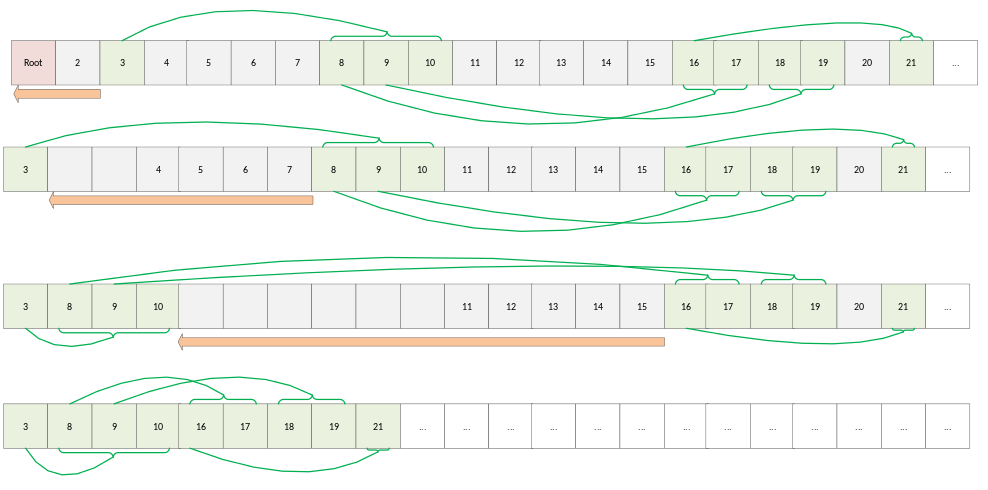
\includegraphics[width=\textwidth]{Optimisations/array.png}}
\caption{\label{fig:Defrag}\textit{defragmentation model, the nodes are compacted to the left.}}
\end{figure}
The aim of this method is to use the RAM for only one array instead of using half of it, due to the presence of the \textit{buffer}. This way, the size of the tree is increased by roughly 50\%.

However that second method requires many more updates than expected: 
each time a node is moved, it is required to change the pointer of its parent, if it is the first node. It also require to update the parent pointer of its children. All this greatly increases the number of calls in the memory. In order to solve such a problem, we used another array, \textit{index} which reference the address of each node. When moving one node, it is required to change its reference while the parent and children points to that direction.

While the benefits of such implementation are clear, the time spent compacting greater trees grows much in comparison to the first method. Due to such heavy drawback, the second method has been dropped.

\subsection{Scaling on multi-core machine}

A bench mode (\textit{-b} or \textit{--bench}) has been implemented in order to easily follow the evolution of scaling through the subsequent iterations and improvements. We had access to Rodrigue, an old (2009) 24-core-server. It allowed us to compare the number of simulations done by our algorithm through an increasing number of cores (see the following figures).

\begin{figure}[H] 
\centerline{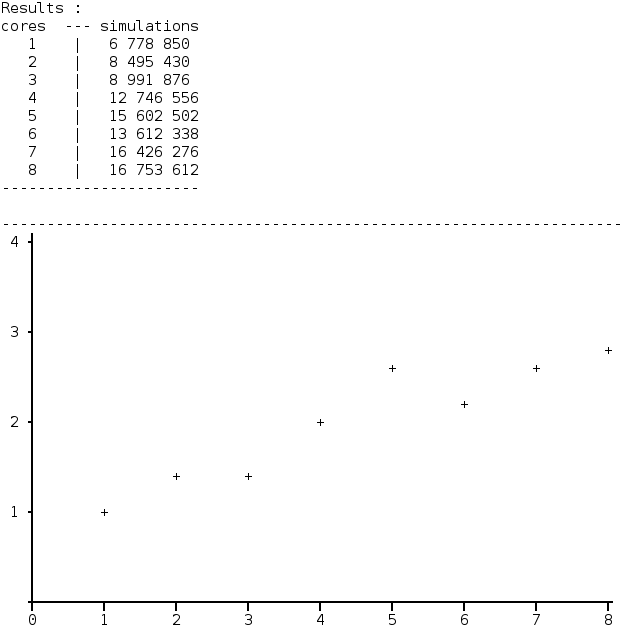
\includegraphics[width=0.8\textwidth]{Optimisations/bench_T1700.png}}
\caption{\label{fig:Defrag}\textit{Bench test on Dell Precision T1700 (4 physical cores, 8 logical cores)}}
\end{figure}

It is shown that the number of simulations doesn't scale well with the number of cores. We expected better results. However these figures are probably due to a poor implementation. We noticed on Rodrigue that from 9 cores, the number of simulations stabilizes. This might be caused because of possible saturation of the memory bus as a result of too much access from the processors and a possible recurring cache invalidation.

\begin{figure}[H] 
\centerline{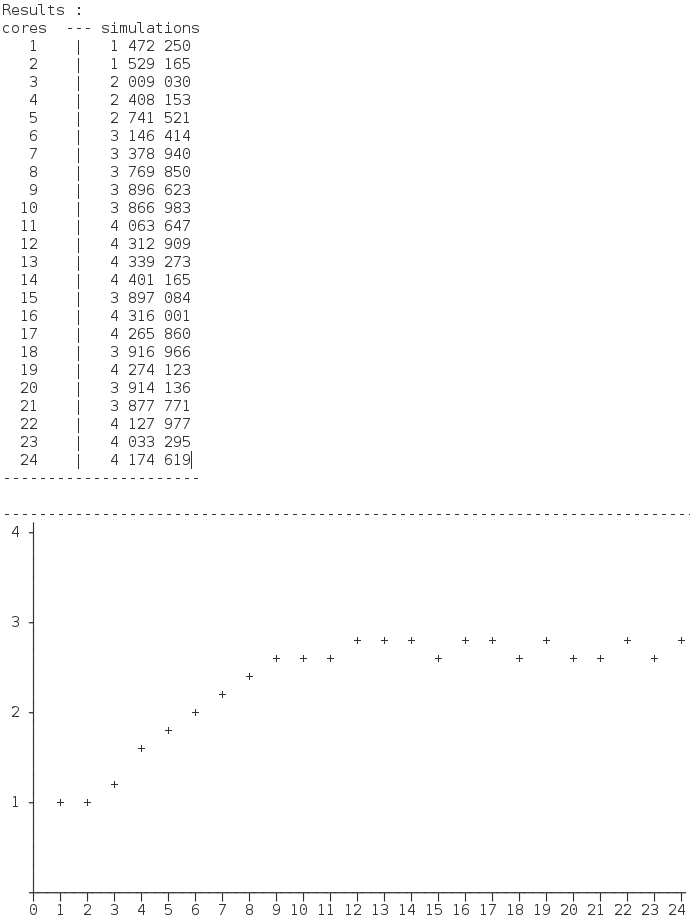
\includegraphics[width=\textwidth]{Optimisations/bench_rodrigue.png}}
\caption{\label{fig:Defrag}\textit{Bench test on Dodrigue (24 physical cores, 24 logical cores)}}
\end{figure}


